\documentclass{article}

\usepackage{multicol}
\usepackage{graphicx}

\title{Regelungstechnik}
\author{Prof. Dröge}
\date{}

\begin{document}

\maketitle

\section*{\centering General}

\newpage
\section*{**.**.2024}
Semester-Anfang muss noch nachgetragen werden

\newpage
 \section*{\centering 15.10.2024}

  x) Regelgröße:
  - die physikalische Größe, die geregelt werden soll. Das bedeutet ein physikalischer Wert in einem gewünschten Maß gehalten wird.

  w) Führungsgröße:
  -

  y) Stellgröße:
  - physikalische Größe, welche die Regelgröße auf eine gewünschte Weise beeinflusst. (Bsp. Volumen Strom)

  e) Regelabweichung:
  - Differenz = Führungsgröße - Regelgröße

  z) Störgröße:
  - Einflüsse die selbst nicht beeinflusst werden können
  - Größen, die eine eingestellte Regelung aus dem Gleichgewicht bringt.

  Regelstrecke:
  - ist das zugrunde liegende System

  Systemarten: (Eingang/Ursache - Ausgang/Wirkung)
  - Intigrator: bsp. Volumenstrom wird in Volumen aufintigriert
  - Verstärker: bsp. Hebel

\newpage
\section*{12.11.2024}
\section*{14.11.2024}
letzten zwei Vorlesungen fehlen noch (müssen wegen krankheit nachgetragen werden)

\newpage
\section*{\centering 19.11.2024}
\subsection*{Wiederholung}
\subsubsection*{Merken:}
\begin{itemize}
	\item Impulsfunktion $\delta (t)$ $\rightarrow$ Gewichtsfunktion $g(t)$
	\item Sprungfunktion $\alpha (t) _{falsche variable kann aber in den Folien nachgeschaut werden}$ $\rightarrow$ Übergangsfunktion $h(t)$
	\item (für die Rücktransformation sollte Partialbruchzerlegung sitzten)
\end{itemize}

\subsubsection*{Operationsverstärker}
(siehe Folien)

\subsubsection*{Bode-Diagram}
(siehe Folien) $\rightarrow$ Selbststudium

\subsubsection*{Übergangs- und Gewichtfunkiton}
(siehe Folien) $\rightarrow$ Selbststudium

\subsubsection*{Übergangs- und Gewichtfunkiton}
(siehe Folien) $\rightarrow$ Selbststudium

\newpage
\subsection*{Teil 2 - Der Regler}
\subsubsection*{Der PID-Regler: der linearer Regler}
PID $\rightarrow$ besteht aus den drei basis Übertragungsgliedern \\
Warum PID und nicht PT1 etc.?: PT1/ PT2 sind langsamer als der P-Anteil des PID \\

Nomenklatur lernen: 
\begin{itemize}
	\item Sprungantwort $\rightarrow$ Übergangsfunktion
	\item Eingangssignal $x_e(t)$ $\rightarrow$ Regel-Abweichung
	\item Ausgangssignal $x_a(t)$ $\rightarrow$ Stellgröße
\end{itemize}

\[
G(s) = V(1+ \frac{1}{sT_N}+ sT_V)
\]
V = Verstärkung
\begin{multicols}{3}
	P-Anteil: lorem $\rightarrow$  1

	\columnbreak
	I-Anteil: Intigration $\rightarrow$ $\frac{1}{sT_N}$

	\columnbreak
	D-Anteil: Differentation $\rightarrow$ $sT_V$ \\
	(Sprungänderung ist im Einschaltmoment unendlich)
\end{multicols}
\begin{center}
	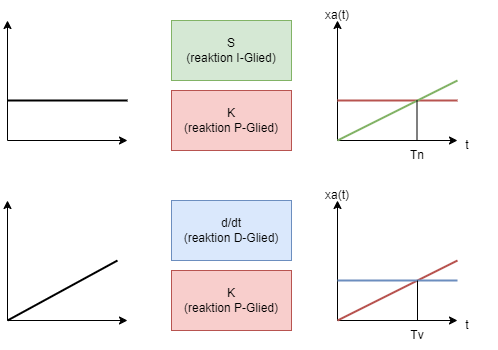
\includegraphics[width=0.6\textwidth]{19_11_2024_reglungstechnik.png}
	% 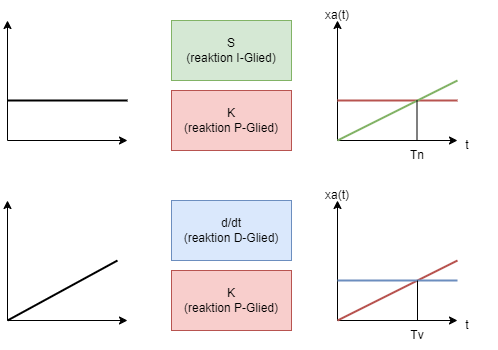
\includegraphics[width=0.5\textwidth]{19_11_2024_reglungstechnik.png}
\end{center}

Typische Anwendung der Glieder: 
\begin{multicols}{3}
	P-Regler nehmen \\
	weil?

	\columnbreak
	PI-Regler \\
	falls P nicht möglich \\
	weil?

	\columnbreak
	PID-Regler \\
	falls PI nicht möglich \\
	weil?
\end{multicols}



\end{document}
